\chapter{Mathematical process model}
\label{chp:MathModel}

\section{Steady state model}
\label{sec:SteadyStateModel}

\subsection{Distillation column}
\label{sec:SSM:dist}

    The distillation column form the heart of the air separation process and their
    operation parameters are crucial in terms of enabling the desired separation.
    While the aspect of heat integration poses is also essential in terms of profitability of
    the process.

    The initial process for production of pure oxygen first developed by Carl von Linde
    and first operated by Linde in 1902 \cite{Barron.1985} consisted of only
    a stripping section, in a way only half a rectification column. The reason for that is
    while it is easy to supply the heat necessary for the reboiler, a heat sink to operate
    a condenser at temperatures of about $95$ $K$ is not readily available on our planet.
    due to that highly pure oxygen could be withdrawn from the bottom of the column, but
    nitrogen was only produces at mediocre purities.

    The breakthrough that enabled operation of a ''full'' column, again developed by Linde in 1910,  was to operate the
    column sections at different pressures. That way the energy needed in the reboiler
    could be withdrawn from the condenser of the other column half. This leads to a
    somewhat inverted construction of the tower in comparison to regular distillation
    units, because the lower section forms the top section in this case and condenser
    and reboiler usually at the top and bottom of a column are combined in a single
    heat exchange unit in the middle of the column. This specialty of the process also
    leads to the need that the absolute values of the energies used in condenser and
    reboiler need to be equal. On terms of modelling the process this also forms a
    considerable challenge. \todo{move process description to different section}

    In this section the working equations used to model the different distillation
    columns in the process, known as the MESH equations, are given. These equations,
    although rather plain at first glimpse, form a set of highly non-linear, highly
    coupled equations. The solutions of these equations is not a trivial
    task for current solution algorithms, whose success is highly dependent on the
    quality of initial guesses provided. Therefore a strategy used for the automated
    generation of such guesses will be described as well.

    \begin{figure}
        \centering
        \begin{subfigure}{0.3\textwidth}
            \centering
            \begin{tikzpicture}[arrow2/.style={line width=0.5pt,->,>=latex,gray},scale=0.52]
    \draw [line width=0.5pt,gray] (1,4.8) -- (-1,4.8) node [above,pos=0.5,black,yshift=-1mm] {\scriptsize 2};
    \draw [line width=0.5pt,gray] (1,-4.8) -- (-1,-4.8) node [above,pos=0.5,black,yshift=-1mm] {\scriptsize N-1};
    \draw [line width=0.5pt,gray] (1,-4.0) -- (-1,-4.0) node [above,pos=0.5,black] {};
    \draw [line width=0.5pt,gray] (1,-3.2) -- (-1,-3.2) node [above,pos=0.5,black] {};
    \draw [line width=0.5pt,gray] (1,-0.8) -- (-1,-0.8) node [above,pos=0.5,black] {};
    \draw [line width=0.5pt,gray] (1,0.0) -- (-1,0.0) node [above,pos=0.5,black] {};
    \draw [line width=0.5pt,gray] (1,0.8) -- (-1,0.8) node [above,pos=0.5,black] {};
    \draw [line width=0.5pt,gray] (1,1.6) -- (-1,1.6) node [above,pos=0.5,black] {};
    \draw [line width=0.5pt,gray] (1,-1.6) -- (-1,-1.6) node [above,pos=0.5,black] {};
    \draw [line width=1pt, rounded corners] (-1.0,2.8) -- (-1.0,5) .. controls (-0.8,5.8) and (0.8,5.8) .. (1.0,5) node (a) [inner sep=0cm , pos=0.5] {} -- (1.0,2.8);
    \draw [arrow] (a) -- (0,6.2) -- (2.5,6.2) node [draw, line width=1pt, pos=1, circle, minimum size=0.9cm, fill=white] {} -- (2.5,4.8) -- (1,4.8) ; % condenser
    \draw [line width=0.5pt] (4,6.5) -- (2.2,6.5) -- (2.6,6.2) -- (2.2,5.9) -- (4,5.9) ;   % heater condenser
    \draw [line width=1pt] (1.0,2.6) .. controls (0.75,2.85) and (0.25,2.85) .. (0.0,2.6) .. controls (-0.25,2.35) and (-0.75,2.35) .. (-1.0,2.6);
    \draw [line width=1pt] (1.0,-2.2) .. controls (0.75,-2.45) and (0.25,-2.45) .. (0.0,-2.2) .. controls (-0.25,-1.95) and (-0.75,-1.95) .. (-1.0,-2.2);
    \draw [line width=1pt] (1.0,2.8) .. controls (0.75,3.05) and (0.25,3.05) .. (0.0,2.8) .. controls (-0.25,2.55) and (-0.75,2.55) .. (-1.0,2.8);
    \draw [line width=1pt] (1.0,-2.4) .. controls (0.75,-2.65) and (0.25,-2.65) .. (0.0,-2.4) .. controls (-0.25,-2.15) and (-0.75,-2.15) .. (-1.0,-2.4);
    \draw [line width=1pt] (1.0,2.6) -- (1.0,-2.2) ;
    \draw [line width=1pt] (-1.0,2.6) -- (-1.0,-2.2) ;
    \draw [line width=1pt, rounded corners] (1.0,-2.4) -- (1.0,-5) .. controls (0.8,-5.8) and (-0.8,-5.8) .. (-1.0,-5) node (b) [inner sep=0cm , pos=0.5] {} -- (-1.0,-2.4) ;
    \draw [arrow] (b) -- (0,-6.2) -- (2.5,-6.2) node [draw, line width=1pt, pos=1, circle, minimum size=0.9cm, fill=white] {} -- (2.5,-4.8) -- (1,-4.8) ;
    \draw [line width=0.5pt] (4,-6.5) -- (2.2,-6.5) -- (2.6,-6.2) -- (2.2,-5.9) -- (4,-5.9) ; % heater reboiler
    \draw [arrow2] (2.0,-4.8) -- (2.0,-4.0) -- (1.0,-4.0) ;
    \draw [arrow2] (2.0,-4.0) -- (2.0,-3.2) -- (1.0,-3.2) ;
    \draw [arrow2] (-2.0,0.8) -- (-2.0,1.6) -- (-1.0,1.6) ;
    \draw [arrow2] (-2.0,0.8) -- (-2.0,0.0) -- (-1.0,0.0) ;
    \draw [arrow2] (-2.0,0.0) -- (-2.0,-0.8) -- (-1.0,-0.8) ;
%    \draw [arrow2] (-2.0,-0.8) -- (-2.0,-1.6) -- (-1.0,-1.6) ;
%    \draw [arrow2] (1.0,-0.8) -- (2.0,-0.8) ;
    \draw [arrow2] (1.0,0.0) -- (2.0,0.0) ;
    \draw [arrow2] (1.0,0.8) -- (2.0,0.8) ;
%    \draw [arrow2] (1.0,1.6) -- (2.0,1.6) ;
    \draw [arrow2] (1.0,-1.6) -- (2.0,-1.6) ;
    \draw [line width=0.5pt,gray] (2.0,0.8) -- (2.0,-1.6) ;
    \draw [line width=0.5pt,gray,dotted] (-2.0,1.6) -- (-2.0,2.2) ;
    \draw [line width=0.5pt,gray,dotted] (-2.0,-0.8) -- (-2.0,-1.4) ;
    \draw [line width=0.5pt,gray,dotted] (2.0,0.8) -- (2.0,1.4) ;
    \draw [line width=0.5pt,gray,dotted] (2.0,-1.6) -- (2.0,-2.2) ;
    \draw [line width=0.5pt,gray,dotted] (2.0,-3.2) -- (2.0,-2.6) ;
    \draw [arrow] (2.5,4.8) -- (4,4.8) ;
    \draw [arrow] (2.5,-4.8) -- (4,-4.8) ;
    \draw [arrow] (-3.0,0.8) -- (-1.0,0.8) ;
    \draw [arrow] (1.0,-0.8) -- (3.0,-0.8) ;
    \node at (2.0,-6.2) {\scriptsize N} ;
    \node at (2.0,6.2) {\scriptsize 1} ;
\end{tikzpicture}

            \label{fig:col_super}
            \caption{column super structure.}
        \end{subfigure}
        \qquad
        \begin{subfigure}{0.6\textwidth}
            \centering
            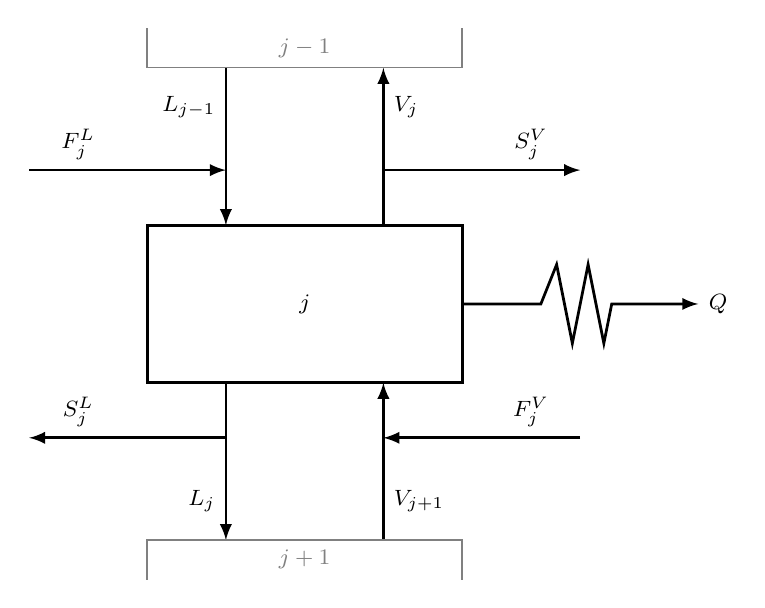
\begin{tikzpicture}[arrow/.style={line width=1pt,->,>=latex}]
	\draw [line width=1pt] (-2,1) rectangle (2,-1) node at (0,0) {\footnotesize $j$};
	\draw [arrow] (-1,3) -- (-1,1) node [pos=0.25, left] {\footnotesize $L_{j-1}$};
 	\draw [arrow] (-3.5,1.7) -- (-1,1.7) node [pos=0.25, above] {\footnotesize $F^L_{j}$};
 	\draw [arrow] (1,1) -- (1,3) node [pos=0.75, right] {\footnotesize $V_{j}$};
 	\draw [arrow] (1,1.7) -- (3.5,1.7) node [pos=0.75, above] {\footnotesize $S^V_{j}$};
 	\draw [arrow] (-1,-1) -- (-1,-3) node [pos=0.75, left] {\footnotesize $L_{j}$};
 	\draw [arrow] (-1,-1.7) -- (-3.5,-1.7) node [pos=0.75, above] {\footnotesize $S^L_{j}$};
	\draw [arrow] (1,-3) -- (1,-1) node [pos=0.25, right] {\footnotesize $V_{j+1}$};
	\draw [arrow] (3.5,-1.7) -- (1,-1.7) node [pos=0.25, above] {\footnotesize $F^V_{j}$};
	\draw [arrow] (2,0) -- (3,0) -- (3.2,0.5) -- (3.4,-0.5) -- (3.6,0.5) -- (3.8,-0.5) -- (3.9,0) -- (5,0,0) node [pos=1, right] {\footnotesize $Q$} ;
    \draw [line width=0.5pt,gray] (-2,-3.5) -- (-2,-3) -- (2,-3) node [pos=0.5, below] {\footnotesize $j+1$} -- (2,-3.5) ; 
    \draw [line width=0.5pt,gray] (-2,3.5) -- (-2,3) -- (2,3) node [pos=0.5, above] {\footnotesize $j-1$} -- (2,3.5) ;
\end{tikzpicture}

            \label{fig:col_stage_super}
            \caption{stage super structure.}
        \end{subfigure}
        \label{fig:col_super_structs}
        \caption{superstructures for column and column stages.}
    \end{figure}
%    \begin{figure}
%        \centering
%        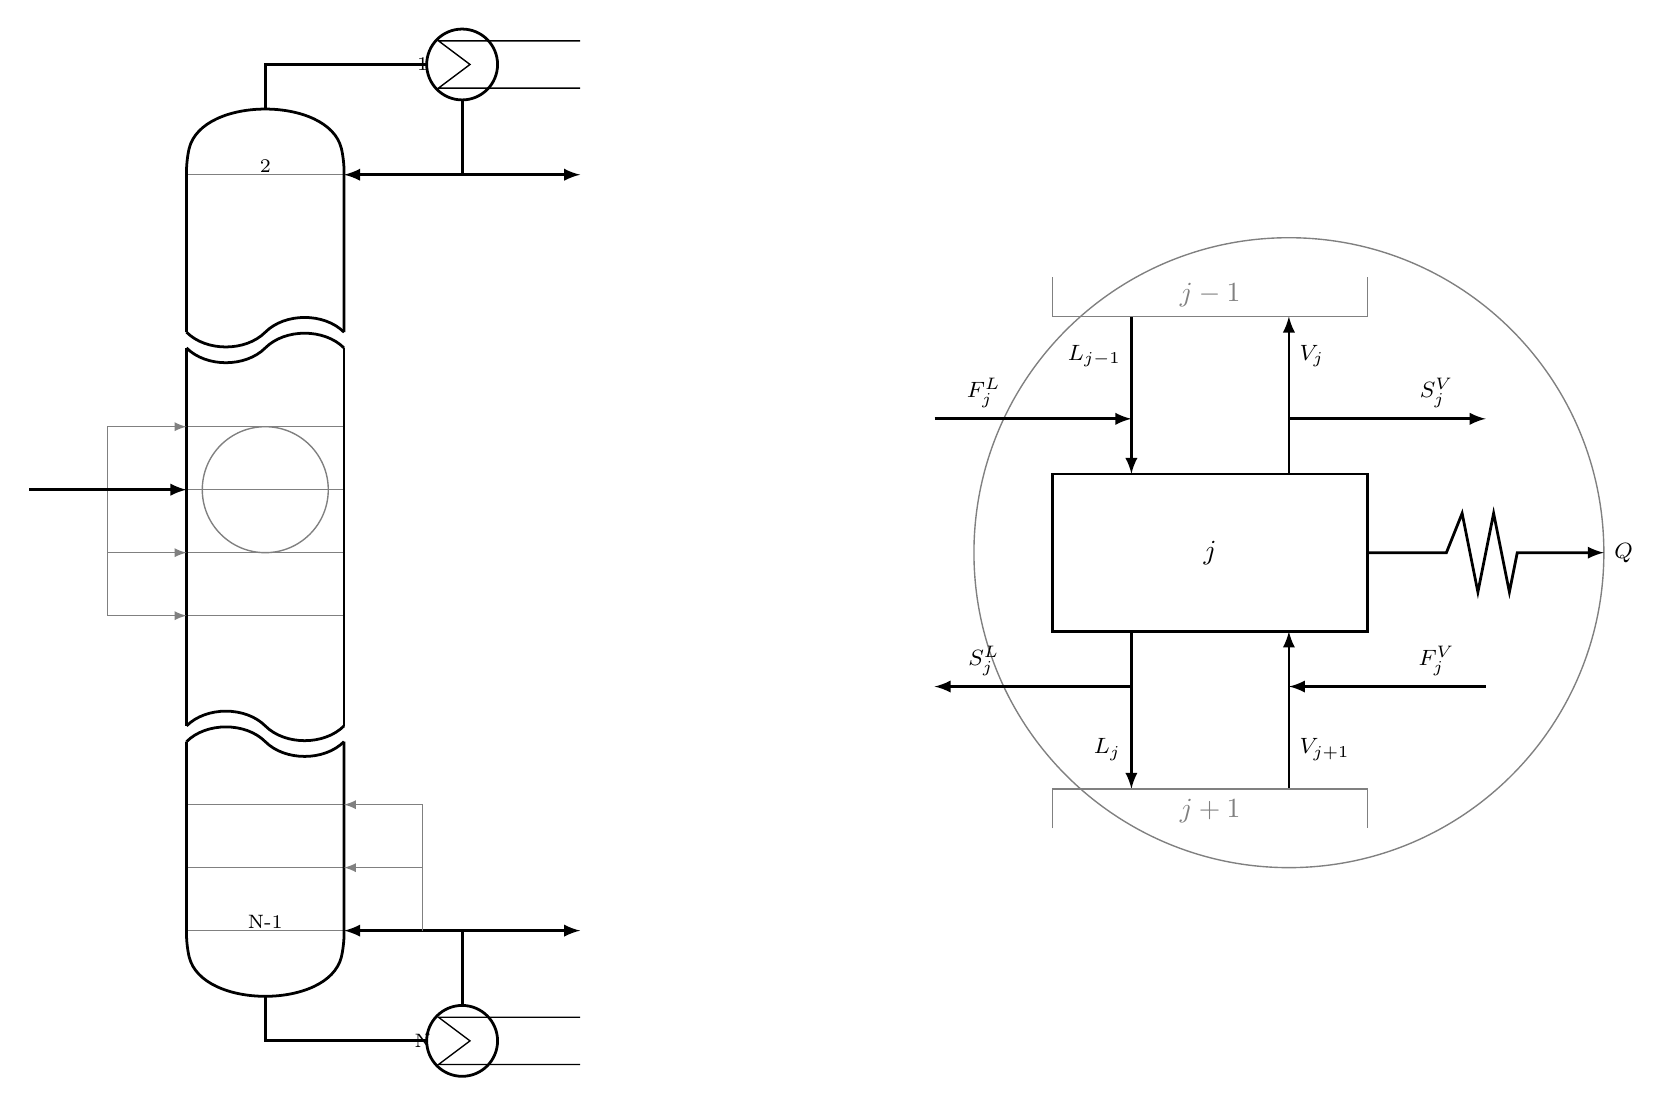
\begin{tikzpicture}[arrow/.style={line width=1pt,->,>=latex},arrow2/.style={line width=0.5pt,->,>=latex,gray}]
    \draw [line width=0.5pt,gray] (1,4.8) -- (-1,4.8) node [above,pos=0.5,black,yshift=-1mm] {\scriptsize 2};
    \draw [line width=0.5pt,gray] (1,-4.8) -- (-1,-4.8) node [above,pos=0.5,black,yshift=-1mm] {\scriptsize N-1};
    \draw [line width=0.5pt,gray] (1,-4.0) -- (-1,-4.0) node [above,pos=0.5,black] {};
    \draw [line width=0.5pt,gray] (1,-3.2) -- (-1,-3.2) node [above,pos=0.5,black] {};
    \draw [line width=0.5pt,gray] (1,-0.8) -- (-1,-0.8) node [above,pos=0.5,black] {};
    \draw [line width=0.5pt,gray] (1,0.0) -- (-1,0.0) node [above,pos=0.5,black] {};
    \draw [line width=0.5pt,gray] (1,0.8) -- (-1,0.8) node [above,pos=0.5,black] {};
    \draw [line width=0.5pt,gray] (1,1.6) -- (-1,1.6) node [above,pos=0.5,black] {};
    \draw [line width=1pt, rounded corners] (-1.0,2.8) -- (-1.0,5) .. controls (-0.8,5.8) and (0.8,5.8) .. (1.0,5) node (a) [inner sep=0cm , pos=0.5] {} -- (1.0,2.8);
    \draw [arrow] (a) -- (0,6.2) -- (2.5,6.2) node [draw, line width=1pt, pos=1, circle, minimum size=0.9cm, fill=white] {} -- (2.5,4.8) -- (1,4.8) ; % condenser
    \draw [line width=0.5pt] (4,6.5) -- (2.2,6.5) -- (2.6,6.2) -- (2.2,5.9) -- (4,5.9) ;   % heater condenser
    \draw [line width=1pt] (1.0,2.6) .. controls (0.75,2.85) and (0.25,2.85) .. (0.0,2.6) .. controls (-0.25,2.35) and (-0.75,2.35) .. (-1.0,2.6); 
    \draw [line width=1pt] (1.0,-2.2) .. controls (0.75,-2.45) and (0.25,-2.45) .. (0.0,-2.2) .. controls (-0.25,-1.95) and (-0.75,-1.95) .. (-1.0,-2.2);
    \draw [line width=1pt] (1.0,2.8) .. controls (0.75,3.05) and (0.25,3.05) .. (0.0,2.8) .. controls (-0.25,2.55) and (-0.75,2.55) .. (-1.0,2.8);
    \draw [line width=1pt] (1.0,-2.4) .. controls (0.75,-2.65) and (0.25,-2.65) .. (0.0,-2.4) .. controls (-0.25,-2.15) and (-0.75,-2.15) .. (-1.0,-2.4);
    \draw [line width=1pt] (1.0,2.6) -- (1.0,-2.2) ; 
    \draw [line width=1pt] (-1.0,2.6) -- (-1.0,-2.2) ;
    \draw [line width=1pt, rounded corners] (1.0,-2.4) -- (1.0,-5) .. controls (0.8,-5.8) and (-0.8,-5.8) .. (-1.0,-5) node (b) [inner sep=0cm , pos=0.5] {} -- (-1.0,-2.4) ;
    \draw [arrow] (b) -- (0,-6.2) -- (2.5,-6.2) node [draw, line width=1pt, pos=1, circle, minimum size=0.9cm, fill=white] {} -- (2.5,-4.8) -- (1,-4.8) ;
    \draw [line width=0.5pt] (4,-6.5) -- (2.2,-6.5) -- (2.6,-6.2) -- (2.2,-5.9) -- (4,-5.9) ; % heater reboiler
    \draw [arrow2] (2.0,-4.8) -- (2.0,-4.0) -- (1.0,-4.0) ;
    \draw [arrow2] (2.0,-4.0) -- (2.0,-3.2) -- (1.0,-3.2) ;
    \draw [arrow2] (-2.0,0.8) -- (-2.0,1.6) -- (-1.0,1.6) ;
    \draw [arrow2] (-2.0,0.8) -- (-2.0,0.0) -- (-1.0,0.0) ;
    \draw [arrow2] (-2.0,0.0) -- (-2.0,-0.8) -- (-1.0,-0.8) ;
    \draw [arrow] (2.5,4.8) -- (4,4.8) ;
    \draw [arrow] (2.5,-4.8) -- (4,-4.8) ;
    \draw [arrow] (-3.0,0.8) -- (-1.0,0.8) ;
    \node at (2.0,-6.2) {\scriptsize N} ;
    \node at (2.0,6.2) {\scriptsize 1} ;
    \node (C) [draw, line width=0.5pt, circle, gray, minimum size=1.6cm] at (0,0.8){} ;
    \node (D) [draw, line width=0.5pt, circle, gray, minimum size=8cm] at (13,0) {} ;
    \draw [line width=1pt] (10,1) rectangle (14,-1) node at (12,0) {$j$};
	\draw [arrow] (11,3) -- (11,1) node [pos=0.25, left] {\footnotesize $L_{j-1}$};
 	\draw [arrow] (8.5,1.7) -- (11,1.7) node [pos=0.25, above] {\footnotesize $F^L_{j}$};
 	\draw [arrow] (13,1) -- (13,3) node [pos=0.75, right] {\footnotesize $V_{j}$};
 	\draw [arrow] (13,1.7) -- (15.5,1.7) node [pos=0.75, above] {\footnotesize $S^V_{j}$};
 	\draw [arrow] (11,-1) -- (11,-3) node [pos=0.75, left] {\footnotesize $L_{j}$};
 	\draw [arrow] (11,-1.7) -- (8.5,-1.7) node [pos=0.75, above] {\footnotesize $S^L_{j}$};
	\draw [arrow] (13,-3) -- (13,-1) node [pos=0.25, right] {\footnotesize $V_{j+1}$};
	\draw [arrow] (15.5,-1.7) -- (13,-1.7) node [pos=0.25, above] {\footnotesize $F^V_{j}$};
	\draw [arrow] (14,0) -- (15,0) -- (15.2,0.5) -- (15.4,-0.5) -- (15.6,0.5) -- (15.8,-0.5) -- (15.9,0) -- (17,0,0) node [pos=1, right] {\footnotesize $Q$} ;
    \draw [line width=0.5pt,gray] (10,-3.5) -- (10,-3) -- (14,-3) node [pos=0.5, below] {$j+1$} -- (14,-3.5) ;
    \draw [line width=0.5pt,gray] (10,3.5) -- (10,3) -- (14,3) node [pos=0.5, above] {$j-1$} -- (14,3.5) ;
\end{tikzpicture}

%        \label{fig:col_com_stage_super}
%        \caption{superstructures for column and column stages.}
%    \end{figure}

    \Reffig{fig:col_super_structs} shows the super structures for a distillation column
    with a single feed and and no side draws (\reffig{fig:col_super}) and a single inner
    column stage (\reffig{fig:col_stage_super}).
    The acronym MESH stands for Material (M), Equilibrium (E), Summation (S) and Enthalpy (H)
    equations which are given below.

%	\paragraph{Mass balance}
%	\Eq{eq:col:MassBalance}{
%		0 = F_j^V + F_j^L + V_{j+1} + L_{j-1} - V_j - S_j^V - L_j - S_j^L
%		\nc{F_j^V}{Vapour feed to tray $j$}{\frac{mol}{s}}
%		\nc{F_j^L}{Liquid feed to tray $j$}{\frac{mol}{s}}
%		\nc{S_j^V}{Vapour side flow from tray $j$}{\frac{mol}{s}}
%		\nc{S_j^L}{Liquid side flow from tray $j$}{\frac{mol}{s}}
%		\nc{V_j}{Vapour flow from tray $j$}{\frac{mol}{s}}
%		\nc{L_j}{Liquid flow from tray $j$}{\frac{mol}{s}}
%	}%

	\paragraph{Material balances}
        The material balances in their most general form for an inner column stage can be written
        as
        \Eqml{eq:col:CompBalance}{
    		0 = \left(V_j + S_j^V\right) \cdot y_{i,j} + \left(L_j + S_j^L\right) \cdot x_{i,j}
                - V_{j+1} \cdot y_{i,j+1} - L_{j-1} \cdot x_{i,j-1} \\ - F_j^V \cdot z^V_{i,j}
                - F_j^L \cdot z_{i,j}^L, \eqannote{i = 1 \dots C, \quad j = 1 \dots N}.
    	}%
        \nc{V_j}{molar vapour flowrate form stage $j$}{\mols}
        \nc{L_j}{molar liquid flowrate form stage $j$}{\mols}
        \nc{y_{ij}}{vapour mole fraction of component $i$ on stage $j$}{-}
        \nc{x_{ij}}{liquid mole fraction of component $i$ on stage $j$}{-}
        \nc{S^L_j}{molar liquid side-draw flowrate form stage $j$}{\mols}
        \nc{S^V_j}{molar vapour side-draw flowrate form stage $j$}{\mols}
        \nc{F^L_j}{molar liquid feed flowrate to stage $j$}{\mols}
        \nc{F^V_j}{molar vapour feed flowrate to stage $j$}{\mols}
        \nc{z^L_{ij}}{liquid mole fraction of liquid feed to stage $j$}{-}
        \nc{z^V_{ij}}{vapour mole fraction of vapour feed to stage $j$}{-}
    
        Here the vapour and liquid phase of the feed to the stage are considered separately.
        While this is not strictly necessary is allows for certain freedoms in terms of modelling
        column operations, as sometimes the vapour fraction of a given feed is actually fed into
        the vapour phase of a stage and therefore effectively in the liquid phase of the stage above.
    
        To facilitate convergence the side draw streams $S_j^V$ and $S_j^L$ are made dimensionless
        by means of the respective vapour and liquid flows on that stage to form the
        vapour
        \Eq{eq:val:vap:strip}{
            s_j^V = \frac{S_j^V}{V_j}, \eqannote{j = 1 \dots N}
        }%
        \nc{s^V_j}{dimensionless vapour side-draw from stage $j$}{-}
        and liquid
        \Eq{eq:val:vap:strip}{
            s_j^L = \frac{S_j^L}{L_j}, \eqannote{j = 1 \dots N}
        }%
        \nc{s^V_j}{dimensionless liquid side-draw from stage $j$}{-}
        stripping factors. Replacing the side-streams in the material balances by their
        corresponding stripping factors yields
        \Eqml{eq:col:CompBalance}{
    		0 = \left(1 + s_j^V\right) \cdot V_j \cdot y_{i,j} + \left(1 + s_j^L\right)
                \cdot L_j \cdot x_{i,j} - V_{j+1} \cdot y_{i,j+1} - L_{j-1} \cdot x_{i,j-1}
                \\ - F_j^V \cdot z^V_{i,j} - F_j^L \cdot z_{i,j}^L,
                \eqannote{i = 1 \dots C, \quad j = 1 \dots N}.
    	}%
        \nc{C}{number of components}{-}
        \nc{N}{number of stages}{-}
    
        As the model is also to be used for optimization purposes further extensions are necessary.
        The location of individual feeds as well as the number of theoretical or real stages of the
        column is to be optimized. To accommodate that need, new variables need, namely the feed
        split $\zeta_{ij}^F$ for feed $i$ to stage $j$ need to be introduced. The split variables are
        integer variables that can take a value of $0$ or $1$. Additionally it is assumed that each
        feed will only be fed to a single stage thus
        \Eq{eq:col:feedsplit}{
            0 = 1 - \sum_{j=1}^N \zeta_{ij}, \eqannote{i = 1 \dots F, \quad j = 1 \dots N},
        }%
        where $F$ denotes the number of feeds, comprised of vapour ($F^V$) and liquid $F^L$ feeds.
    
        In order to optimize the number of stages several superstructures are possible. One can
        optimize the reboiler reflux location and condenser reflux location or each single one
        along with the feed and side draw locations. The stage number is then changed as all stages
        between condenser or reboiler reflux are effectively rendered inactive. The solution of
        the mass and energy balances for each respective stages becomes trivial as only one single
        vapour or liquid stream enters and exits the stage. While the choice if condenser and or reboiler
        reflux is optimized is somewhat arbitrary some studies have shown \cite{Grossmann.2005} that
        the strategy of optimizing only feed location and reboiler reflux location possesses some
        numerical advantages in terms of performance of the solution algorithm.
    
        With the newly introduced split variables for liquid $\zeta^L_{ij}$ and vapour $\zeta^V_{ij}$
        as well as the reboiler reflux $\zeta^R_j$ and the liquid $\zeta^{SL}_{ij}$ and vapour $\zeta^{SV}_{ij}$
        side draws, the material balances can be written as
        \Eqml{eq:col:CompBalance_opt}{
    		0 = \left(1 + s_j^V\right) \cdot V_j \cdot y_{i,j} + \left(1 + s_j^L\right)
                \cdot L_j \cdot x_{i,j} - V_{j+1} \cdot y_{i,j+1} \\ \hfill - L_{j-1} \cdot x_{i,j-1}
                - \sum_{k=1}^{F^V} \zeta_{kj} \cdot F_j^V \cdot z^V_{i,j} - \sum_{l=1}^{F^L}%
                \zeta_{lj} \cdot F_j^L \cdot z_{i,j}^L - \zeta^R_j \cdot V_N \cdot y_{iN}, \hfill%
                \\ \eqannote{i = 1 \dots C, \quad j = 1 \dots N, \quad k = 1 \dots F^V, \quad l = 1 \dots F^L}.
    	}%
        \nc{\zeta^{L}_{ij}}{splitting variable for liquid feed $i$ on stage $j$}{-}
        \nc{\zeta^{V}_{ij}}{splitting variable for vapour feed $i$ on stage $j$}{-}
        \nc{\zeta^{SV}_{ij}}{splitting variable for vapour side draw $i$ on stage $j$}{-}
        \nc{\zeta^{SL}_{ij}}{splitting variable for liquid side draw $i$ on stage $j$}{-}
        \nc{\zeta^{R}_{j}}{splitting variable for reboiler reflux on stage $j$}{-}
    
        Furthermore to be able to optimize side draws, the stripping factors have to be reformulated
        accordingly
        \Eq{eq:val:vap:strip_opt}{
            s_j^V = \frac{\sum_{i=1}^{S^V} \zeta^{SV}_{ij} S_j^V}{V_j}, \eqannote{j = 1 \dots N, \quad i = 1 \dots S^V},
        }%
        \Eq{eq:val:liq:strip_opt}{
            s_j^V = \frac{\sum_{i=1}^{S^L} \zeta^{SL}_{ij} S_j^L}{L_j}, \eqannote{j = 1 \dots N, \quad i = 1 \dots S^L}.
        }%

    \paragraph{Equilibrium equations}
        The equilibrium equations are given by
        \Eq{eq:col:Kxy}{
            y_{ij} = K_{ij} \cdot x_{ij}, \eqannote{i = 1 \dots C, \quad j = 1 \dots N}.
    	}%
        \nc{K_{ij}}{equilibrium ratio of component $i$ on stage $j$}{-}
    
        Where the equilibrium ratio $K_{ij}$ is computed from the relations that describe
        a vapour liquid equilibrium (VLE).
    
        A vapour and liquid phase are in equilibrium, when the fugacities in the vapour $f_i^V$
        and liquid $f_i^L$ phase for each species $i$ are equal \cite{AndreasPfennig.2003}
        \Eq{eq:col:fug}{
            f_i^V = f_i^L, \eqannote{i = 1 \dots C}.
    	}%
        \nc{f_i^V}{vapour fugacity}{-}
        \nc{f_i^L}{liquid fugacity}{-}
    
        This can also be written in terms of the, liquid activity coefficient $\gamma_i$,
        the pointing factor $F_{Pi}$, the reference vapour fugacity coefficient $\varphi_i$,
        the vapour pressure $p^S_i$ as well as the system pressure $p$ along with the vapour and
        liquid molar fractions
        \Eq{eq:col:fug_ext}{
            \gamma_i \, F_{Pi} \, \varphi^0_i \, p^S_i \, x_i = \varphi_i \, p \, y_i, \eqannote{i = 1 \dots C}.
    	}%
        \nc{\gamma_i}{liquid activity coefficient of component $i$}{-}
        \nc{\varphi^0_i}{reference vapour fugacity coefficient of component $i$}{-}
        \nc{\varphi_i}{vapour fugacity coefficient of component $i$}{-}
        \nc{p^S_i}{vapour pressure of component $i$}{Pa}
        \nc{p}{system pressure}{Pa}
        \nc{F_{Pi}}{compressibility factor of component $i$}{-}
    
        By reformulating \refeq{eq:col:fug_ext} an expression for the equilibrium ratios
        can be derived
        \Eq{eq:col:fug_ext}{
            y_i = \underbrace{\frac{\gamma_i \, F_{Pi} \, \varphi^0_i \, p^S_i}{\varphi_i \, p}}_{K_i}
                x_i, \eqannote{i = 1 \dots C}.
    	}%
    
        The equations to determine the quantities used when computing the equilibrium ratios are by
        themselves functions of temperature, pressure, and vapour as well as liquid molar fractions.
        They are further discussed in \refsec{sec:peng-rob}. It therefore becomes evident that the
        equilibrium ratios are a major source  non-linearities in the MESH equations.

	\paragraph{Enthalpy balances}
        The enthalpy balances can again be written using the previously defined stripping factors
        and splitting variables
    	\Eqml{eq:col:EnergyBalance}{
    		0 = \left(1 + s_j^V\right) \cdot V_j \cdot h^V_{j} + \left(1 + s_j^L\right)
                \cdot L_j \cdot h^L_{j} - V_{j+1} \cdot h^V_{j+1} \\ \hfill - L_{j-1} \cdot h^L_{j-1}
                - \sum_{k=1}^{F^V} \zeta_{kj} \cdot F_k^V \cdot h^{FV}_{j} - \sum_{l=1}^{F^L}
                \zeta_{lj} \cdot F_j^L \cdot h^{FL}_{j} - \zeta^R_j \cdot V_N \cdot h^V_{N}, \hfill
                \\ \eqannote{i = 1 \dots C, \quad j = 1 \dots N, \quad k = 1 \dots F^V, \quad l = 1 \dots F^L}.
    	}%
        \nc{h^V_j}{molar vapour enthalpy on stage $j$}{\molenth}
        \nc{h^L_j}{molar liquid enthalpy on stage $j$}{\molenth}
        \nc{h^{FV}_j}{molar vapour feed enthalpy to stage $j$}{\molenth}
        \nc{h^{FL}_j}{molar liquid feed enthalpy to stage $j$}{\molenth}

    \paragraph{Condenser and reboiler}
        \begin{figure}
            \centering
            \begin{subfigure}{0.45\textwidth}
                \centering
                \begin{tikzpicture}[scale=0.7]
	\draw [line width=1pt] (-2,1) rectangle (2,-1) node at (0,0) {\footnotesize $1$};
 	\draw [arrow] (1,1) -- (1,3) node [pos=0.75, right] {\footnotesize $V_{1}$};
 	\draw [arrow] (-1,-1) -- (-1,-3) node [pos=0.75, left] {\footnotesize $L_{1}$};
 	\draw [arrow] (-1,-1.7) -- (-3.5,-1.7) node [pos=0.75, above] {\footnotesize $S^L_{1}$};
	\draw [arrow] (1,-3) -- (1,-1) node [pos=0.25, right] {\footnotesize $V_{2}$};
	\draw [arrow] (2,0) -- (3,0) -- (3.2,0.5) -- (3.4,-0.5) -- (3.6,0.5) -- (3.8,-0.5) -- (3.9,0) -- (5,0,0) node [pos=1, right] {\footnotesize $Q^c$} ;
    \draw [line width=0.5pt,gray] (-2,-3.5) -- (-2,-3) -- (2,-3) node [pos=0.5, below] {\footnotesize $2$} -- (2,-3.5) ;
\end{tikzpicture}

                \label{fig:col_condenser}
                \caption{condenser stage.}
            \end{subfigure}
            \begin{subfigure}{0.45\textwidth}
                \centering
                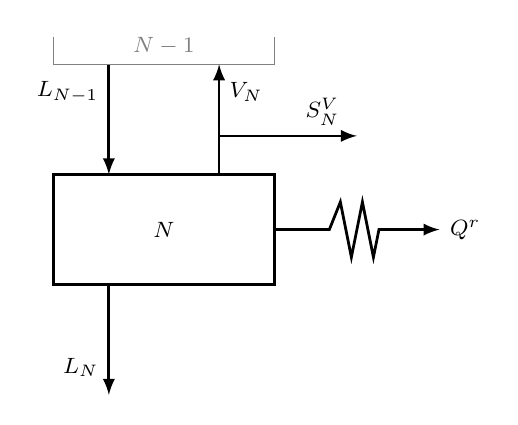
\begin{tikzpicture}[arrow/.style={line width=1pt,->,>=latex},scale=0.7]
	\draw [line width=1pt] (-2,1) rectangle (2,-1) node at (0,0) {\footnotesize $N$};
	\draw [arrow] (-1,3) -- (-1,1) node [pos=0.25, left] {\footnotesize $L_{N-1}$};
 	\draw [arrow] (1,1) -- (1,3) node [pos=0.75, right] {\footnotesize $V_{N}$};
 	\draw [arrow] (1,1.7) -- (3.5,1.7) node [pos=0.75, above] {\footnotesize $S^V_{N}$};
 	\draw [arrow] (-1,-1) -- (-1,-3) node [pos=0.75, left] {\footnotesize $L_{N}$};
	\draw [arrow] (2,0) -- (3,0) -- (3.2,0.5) -- (3.4,-0.5) -- (3.6,0.5) -- (3.8,-0.5) -- (3.9,0) -- (5,0,0) node [pos=1, right] {\footnotesize $Q^r$} ; 
    \draw [line width=0.5pt,gray] (-2,3.5) -- (-2,3) -- (2,3) node [pos=0.5, above] {\footnotesize $N-1$} -- (2,3.5) ;
\end{tikzpicture}

                \label{fig:col_reboiler}
                \caption{reboiler stage.}
            \end{subfigure}
        \end{figure}
    
        Condenser and reboiler are modeled more or less as regular column stages. However they possess
        certain specialties that are explicitly considered in the column model. For one it is assumed
        that no feeds enter the reboiler and condenser stage. Furthermore no vapour side stream is
        drawn from the condenser stage and no liquid side stream from the reboiler stage.
    
        Additionally the condenser stage needs to examined a little further. In terms of operations
        several assumptions can be made for the condenser. In general one can distinguish a total,
        partial vapour and partial vapour liquid condenser. For the total condenser all vapour that
        enters the respective stage is condensed and only liquid product is drawn (here modeled as
        a side draw). The partial vapour condenser condenses only the vapour the is fed back into
        the column and all product that is drawn is gaseous. The partial vapour liquid condenser
        denotes the most general case, where part of the incoming vapour is condensed and product
        ist drawn as vapour and liquid. The most important thing to consider in these different cases,
        is that while in both partial condensers a vapour liquid equilibrium takes place, due to the
        absence of vapour the same does not hold for the total condenser. To accommodate that fact
        the MESH equations have to be adjusted \cite{Naphtali.1971}. While the material and energy
        balances remain unchanged the equilibrium equations have to be altered. First the vapour and
        liquid compositions are set equal for all but one component
        \Eq{eq:col:total}{
            x_{i1} = y_{i1} \eqannote{i = 1 \dots C-1}, 
        }%
        and the condenser temperature is determined by the bubble point equation 
        \Eq{eq:col:bub}{
            0 = 1 - \sum_i K_{i1} \cdot x_{i1} \eqannote{i = 1 \dots C}.
        }%
        
        When implementing the model in a process simulator it is sensible to consider, that due to 
        the limited accuracy of computers the omitted component in \refeq{eq:col:total} needs to 
        a non-trace component in the condenser stage. The implemented model therefore as to specify
        such a component when a total condenser is chosen to avoid numerical difficulties. 
        
        In practice it is highly unlikely, that the exact amount of energy required to condensate all 
        liquid will be drawn from the condenser. More likely, if all vapour is condensed, a little more
        energy will be withdrawn and slightly sub-cooled liquid will leave the condenser. Therefore 
        the model includes the possibility to specify a degree of sub-cooling $T^{sub}$ which will be 
        considered when calculating the equilibrium ratios. 
        
    \subsubsection{Specifications}

    \subsubsection{Column initialization}
        As mentioned before the solution of the MESH equations can pose a considerable problem
        to numerical solvers. It is therefore necessary to supply the solver with feasible
        estimates for the involved variables that can be used as an initial guess to facilitate
        convergence of the process model. A lot of effort has been spend to formulate robust strategies
        to initialize distillation column models. One of the most prominent is the so called
        Inside-Out algorithm first introduced by Boston and Sullivan \cite{Boston.1974}. Within this
        algorithm an inner and outer iterative loop are employed. Within the outer loop approximate
        parameters for simplified models of phase equilibrium and enthalpy are computed by rigorous
        thermodynamic models and guesses for stage temperatures and concentrations. Within the
        inner loop new stage temperatures and concentrations are by solving the MESH equations
        using the simplified thermodynamic models. Once the inner loop converges the simplified
        model parameters are updated within the outer loop by means of the newly calculated
        temperatures and concentrations. This algorithm converges in many cases even for very poor initial
        guesses and has been extended to handle complex columns with side-draws and even reactive
        distillation \cite{BOSTONJ.F..}. It is still in use in the process simulator \aspen.
        However as it is used within an modular algorithmic environment it is not applicable
        to equation based simulators such as \gproms.

        More recently other approaches have been published to attain improved initial guesses.
        Fletcher and Morton \cite{Fletcher.2000} proposed the solution of a column model at
        infinite reflux and zero feed flow rate. This leads to a much simplified model which can
        be solved more easily. The computed purities and stage numbers can give valuable insight
        into the process model. As this approach relies on the solution of a simplified model
        and has no algorithmic elements, it can be implemented in equation based process simulators.

        Another strategy that has been successfully applied to zeotropic and azeotropic mixtures
        relies on solving the column model for the limiting case of the adiabatic column \cite{Barttfeld.2002}.
        The adiabatic column in this case is the column with the minimal entropy production in a real column.
        To avoid entropy production all streams that come in contact must be in equilibrium. To achieve this
        the column would have to employ an infinite number of stages and have an infinite number of
        heat exchangers along its length. The adiabatic column then uses only two heat exchanger in the
        condenser and reboiler stage and assumes a pinch point at the feed stage. \todo{elaborate on adiabatic column}

        Furthermore a much simpler approach has proven adequate for many applications \cite{Henley.op.2011}
        which is also employed as a starting point in this work.
        There feed properties are used as initial guesses. First a linear temperature profile form the boiling
        temperature to dew temperature of the feed is used to initialize temperatures, whereas a simple flash
        at average column pressure and feed temperature yields a vapour and liquid concentration that which is
        used as uniform profile for every column stage. However as the feed might be sub-cooled liquid or
        super-heated vapour the TP-Flash is replaced by a specified vapour fraction. As vapour fraction
        for the flash initial estimates of the vapour and liquid flow rates at the top and bottom of the
        column are used. The stage-wise molar flow-rates are computed from the constant molal overflow
        assumption.

        While this approach leads to model convergence in many cases, it is not entirely robust.
        While the system considered in this case displays only moderate non-idealities it is highly cupeled.
        Especially the low pressure column (LPC) has multiple feeds and side draws, which leads to non-convergence
        if the aforementioned initialization strategy is employed. However the fact that the system is
        not highly non-ideal can be exploited. Whenever the K-values are not too much dependent on mixture
        composition an intermediate step can be used to refine concentration guesses. The constant molal
        overflow assumption is retained and the equilibrium ratios are computed based on the initial guesses
        from the first stage. The component balance is then reformulated only in terms of liquid component
        flow-rates $l_{ij}$

        \Eqml{eq:init:compbalance}{
            0 = \left((1+s_j^V) \cdot K_{ij} \cdot \frac{V_j}{L_j} + (1+s_j^L) \right) \cdot l_{ij}
                - \frac{V_{j+1}}{L_{j+1}} \cdot K_{ij+1} \cdot l_{ij+1} - l_{ij-1}
                \\ - F_j^V \cdot z^V_{i,j} - F_j^L \cdot z_{i,j}^L,
                \eqannote{i = 1 \dots C, \quad j = 1 \dots N}.
        }%
        \nc{l_{ij}}{liquid molar flowrate of component $i$ from stage $j$}{\mols}
        \nc{v_{ij}}{vapour molar flowrate of component $i$ from stage $j$}{\mols}

        \refeq{eq:init:compbalance} is linear in the liquid component flow rates. Furthermore vapour component
        flow rates are substituted in the linear component balance and can be computed by

        \Eq{eq:init:vapflow}{
            0 = v_{ij} - K_{ij} \cdot \frac{V_j}{L_j} \cdot l_{ij} \eqannote{i = 1 \dots C, \quad j = 1 \dots N}.
        }%

        On of the reasons \refeq{eq:init:compbalance} is formulated in terms of component flow rates rather
        than molar fractions, is that the molar fraction computed in that manner would not be normalized. If
        the mole fractions are computed from the component flow rates normalization is implicitly given

        \Eq{eq:init:liqmolefrac}{
            x_{ij} = \frac{l_{ij}}{\sum_k^C l_{kj}} \eqannote{i = 1 \dots C, \quad j = 1 \dots N}.
        }%
        \Eq{eq:init:vapmolefrac}{
            y_{ij} = \frac{v_{ij}}{\sum_k^C v_{kj}} \eqannote{i = 1 \dots C, \quad j = 1 \dots N}.
        }%

\subsection{Multi stream heat exchanger}

\subsection{Compressor / expander}
	\stdfig{pgfplots/Compressor}{Compressor model.}{fig:Compressor}{h}

	\paragraph{Mass and component balances}
	\Eq{eq:comp:MassBalance}{
		0 = F^{in} - F^{out}
	}%
	\Eq{eq:comp:CompBalance}{
		0 = z_i^{in} - z_i^{out}
	}%

	\paragraph{Isentropic work}
	\Eq{eq:comp:SInOut}{
		S^{in}(T^{in}, p^{in}, z_i^{in}) = S^{out}(T_S^{out}, p^{out}, z_i^{out})
	}%
	\Eq{eq:comp:IsentropicWork}{
		W_S = F^{in} \cdot H^{in}(T^{in}, p^{in}, z_i^{in}) - F^{out} \cdot H^{out}(T_S^{out}, p^{out}, z_i^{out})
	}%

	\paragraph{Compression work}
	\Eq{eq:comp:WEta}{
		W \cdot \eta^C = W_S
	}%
	\Eq{eq:comp:CompressionWork}{
		W_S = F^{in} \cdot H^{in}(T^{in}, p^{in}, z_i^{in}) - F^{out} \cdot H^{out}(T^{out}, p^{out}, z_i^{out})
	}%

	\paragraph{Pressure drop}
	\Eq{eq:comp:PressureDrop}{
		p^{out} = p^{in} + \Delta p
	}%
	
\subsection{Centrifugal pump}
	
	\paragraph{Cost estimation}
		The cost for the pump excluding the motor can be approximated by
		\Eq{eq:pump:CostPump}{
			C_B & = \exp \left[ 9.7171 - 0.6019 \ln[S] + 0.0519 (\ln[S])^2 \right] \eqannote{40 \leq S \leq 100000}\\
			C_p & = f_T \, f_M \, C_B.
		}
		The cost for the centrifugal pump is approximated by the value $S = Q \cdot \sqrt{H} $, where
		$Q$ denotes the volume flow through the pump in gallons per minute $[gpm]$ and $H$ the
		pump head in $[ft]$.
		
		The costs given above is excluding the motor needed. It is then estimated separately. In this
		case the specific quantity is the power consumption $P_C$ needed for the desired stream transport.
		
		\Eqml{eq:pump:CostMotor}{
			C_B  = \exp\big[ 5.8259 + 0.13141 \ln[P_C] + 0.053255 (\ln[Pc])^2 \\
				 + 0.028628 (\ln[P_C])^3 - 0.0035549 (\ln[P_C])^4 \big]
		}	

	\todo[inline]{add formulas for vapour fraction}
	\todo[inline]{check if . or , are used for decimals ...}
\subsubsection{Expander}

\subsubsection{Condenser}

\subsection{Reboiler}

	\stdfig{pgfplots/Reboiler}{Reboiler model.}{fig:Reboiler}{h}

	\paragraph{Mass balance}
	\Eq{eq:reboil:MassBalance}{
		0 = F - V - L
	}%

	\paragraph{Component balance}
	\Eq{eq:reboil:CompBalance}{
		0 = F z_j - V y_j - L x_j
	}%

	\paragraph{Pressure drop}
	\Eq{eq:reboil:PressureDrop}{
		p^R = p^{in} + \Delta p
	}%

\subsection{Heater}

	\stdfig{pgfplots/Heater}{Heater model.}{fig:Heater}{h}

	\paragraph{Mass and component balances}
	\Eq{eq:comp:MassBalance}{
		0 = F^{in} - F^{out}
	}%
	\Eq{eq:comp:CompBalance}{
		0 = z_i^{in} - z_i^{out}
	}%
	
	\paragraph{Pressure drop}
	\Eq{eq:reboil:PressureDrop}{
		p^R = p^{in} + \Delta p
	}%
	
	\todo[inline]{add formulas for vapour fraction}
		
\subsubsection{Pump}

\subsubsection{Separator}

\subsubsection{Joule-Thompson valve}

\subsection{Splitter}
	\stdfig{pgfplots/Splitter}{Splitter model}{fig:Splitter}{h}
	
	\paragraph{Mass and component balances}
	\Eq{eq:comp:MassBalance}{
		0 = F^{in} - \sum_i^N F^{in} \zeta_i
	}%
	\Eq{eq:comp:CompBalance}{
		0 = z_i^{in} - z_i^{out}
	}%
	
	\paragraph{Energy balance}
	\Eq{eq:comp:MassBalance}{
		0 = F^{in} H^{in}(T^{in}, p^{in}, z_i^{in}) - \sum_j^N F_j^{out} H^{out}(T^{out}, p^{out}, z_i^{out})
	}%
	
	\paragraph{Pressure drop}
	\Eq{eq:reboil:PressureDrop}{
		p^{out} = p^{in} + \Delta p
	}%

	\todo[inline]{add formulas for vapour fraction}

\subsubsection{Peng-Robinson Equation of State}
\label{sec:peng-rob}
	
\section{Economic models}
\label{sec:EconModel}
	As discussed earlier economic consideration play a major role in process design. In order to account
	for the process economics the cost of the process to be implemented needs to be estimated at the design
	level. However as limited information is available estimation methods have to be employed. In
	\refsec{chp:ProcesEconomics} the general approach for cost estimation of process equipment was
	introduced, where a specific value such as heat-exchange area or vessel size is used to approximate
	equipment cost. However for more specific units extended models are available, where statistical
	data is employed to yield a more realistic fit to cost data. The cost functions and correction
	factors presented in this chapter are, if not stated otherwise, taken from \cite{Seider.2010}.
	Also unless otherwise stated the unit cost is given for the year 2006 ($CE = 500$).
	
	\subsection{Destillation column}
		Out of all the process equipment the distillation column probably is the most elaborate
		unit. It also poses the greatest challenges when it comes to finding an appropriate
		estimate for its cost. This is die to the fact that the column in itself is rather
		large and complex. To properly operate a column the vessel needs to have numerous
		valves, scaffolding and several manholes. Due to its size further factors come into
		play that need not to be considered for the other relatively small units. Those location
		dependent factors might include resilience towards earthquakes, the ability to withstand
		close winds or intensive ambient temperatures. However as the scope of this work explicitly
		focuses on early design stages those location specific influences will be disregarded
		to arrive at simpler models for cost estimation.
		
		\subsubsection{Vertical tower}
			The cost for the vessel $C_V$ which is to be vertically erected vertically is dependent
			on teh weight fo the weight $W$ ($[lbs]$) of the vessel. This includes valves, manholes and
			other details directly connected with the tower. However the cost for ladders,
			platforms and railings necessary to properly operate the column are calculated
			separately
			\Eq{eq:cost:column:column}{
				C_p = f_M \, C_V + C_{PL}.
			}
			
			The correlated equation for the cost of the tower is given by
			\Eq{eq:cost:column:vessel}{
				C_V = \exp\big\{ 7.2756 + 0.18255 \cdot \ln[W] + 0.02297 \cdot \pow{\ln[W]}{2} \big\}, \eqannote{9000 \leq W \leq 2.5 \cdot 10^6}.
			}
			
			To the cost of the tower, the cost of the surrounding support structure ist added. It is dependent
			on the inner diameter of the vessel ($D_i$) as well as the so called tangent to tangent length ($L$).
			This denotes the length of the tube that makes up the vessel excluding the spherical domes that
			close the column on each side. With that the additional cost is then computed by
			\Eq{eq:cost:column:support}{
				C_{PL} = 300.9 \cdot \pow{D_i}{0.63316} \cdot \pow{L}{0.80161}.
			}
			
		\subsubsection{Weight}
			As can be seen from the above correlations the weight of the column is a determining factor
			for the estimated and actual cost. Therefore some thought should be put into how this can
			be determined, when the final design is unknown. Again several correlations have been applied
			to real life units which yield satisfactory results. In general the weight of the empty vessel
			can be computed by determining the volume of the material and multiplying it with its density ($\varrho$)
			\Eq{eq:cost:column:weight}{
				W = \pi (D_i + t_s)(L + 0.8 \cdot D_i) t_s \cdot \varrho.
			}
			The term $0.8 D_i$ is included to approximate the weight of the domes, whereas $t_s$ is the shell
			thickness. To determine how thick the walls of the shell need to be the ASME pressure vessel code
			formula is often applied
			\Eq{eq:cost:column:wallthickness}{
				t_s = \frac{P_d \, D_i}{2 \, S \, E - 1.2 P_d}.
			}
			Where the maximal allowable stress $S$, which the chosen material can withstand at
			process conditions is multiplied by the fractional weld efficiency $E$ to regard the effects
			of the manufacturing process on the material strength. To ensure an error on the side of
			caution the design pressure $P_d$ is calculated from the actual operating pressure $P_o$
			by means of
			\Eq{eq:cost:column:designpressure}{
				P_d = \exp\big\{ 0.60600 + 0.91615 \cdot \pow{\ln[P_o]}{} + 0.0015655 \cdot \pow{\ln[P_o]}{2}
			}
			It is important to consider, that the maximum allowable stress especially needs to take into account
			the operating temperature of the distillation process, as it might have significant effects.
			
			Furthermore the given formulas only apply to pressures above ambient conditions. Thus low pressure
			or vacuum distillation is not covered by the presented formulas.
			
		\subsubsection{Column internals}
			While internal support structures are already considered by the equations given above, the
			internals responsible to ensure product separation are not. Those make up a very significant
			amount of the total column cost and are available .
	
	\subsection{Centrifugal pump}
		Pumps are among the most common units of process equipment. While there are several different
		kinds of pumps that can be used, the centrifugal pump is one of the most popular choices and
		denotes a very likely choice for the process conditions considered in this application. Hence
		other pump types will not be considered at this point.
		
		\subsubsection{Pump}
			In terms of operations pumps are best described by the volumetric flow transported $Q$ as
			well as the pump head $H$, the hight that needs to be overcome. Data taken from the company
			Mosanto was used to correlate the pump cost to a specific value
			\Eq{eq:cost:pump:SpecVal}{
				S = Q \sqrt{H}.
			}
			As a reference unit the base price $C_B$ is estimated for a cast iron single-stage
			vertically split case at 3600 $rpm$
			\Eq{eq:cost:pump:PumpWOMotor}{
				C_B = \exp \left\{ 9.7171 - 0.6019 \cdot \ln[S] + 0.0519 (\ln[S])^2 \right\},
					\eqannote{400 \leq S \leq 100000}.
			}
			
			The most influential addition factors for the pump price are the material, which is accounted
			for in the material factor $f_m$, as well as the rotation, case split orientation (horizontal
			and vertical), the number of stages, covered flow rate range, pump head range and maximum
			motor power, which are all agglomerated in the type factor $f_T$. Values for these factors
			are given in \reftab{tab:pump:Type} and \reftab{tab:pump:Material}.
			
			\stdtab{Tables/PumpFactorsType}{Pump type factors \cite{Seider.2010}.}{tab:pump:Type}
			\stdtab{Tables/PumpFactorsMaterial}{Pump material factors \cite{Seider.2010}.}{tab:pump:Material}
			
		\subsubsection{Electric motor}
			Separately from the pump itself the motor to drive the compression is considered. While the
			volumetric flow and the pump head certainly are valid choices to correlate motors for pumps
			especially, the power consumption is a more general specific value
			\Eq{eq:cost:pump:MotorPowerConsumption}{
				P_C = \frac{P_T}{\eta_P \eta_M} = \frac{P_B}{\eta_M}
			}
			
			It can be calculated from the theoretic power of the pump $P_T$ and the efficiencies $\eta_P$
			$\eta_M$. While an estimate for the expected power consumption might be already available at
			rather early design stages, the efficiencies will have to be correlated as well if resorting
			to average values is considered too coarse. Those correlations rely on the volumetric flow in
			gallons per minute ([gpm]) and the brake horse power $P_B = \frac{P_T}{\eta_P}$.
			
			\Eq{eq:cost:pump:MotorEfficiancyP}{
				\eta_P = -0.316 + 0.24015 \cdot \ln[Q] - 0.01199 \cdot (\ln[Q])^2 \eqannote{50 \leq Q \leq 5000}
			}
			\Eq{eq:cost:pump:MotorEfficiancyM}{
				\eta_M = 0.80 + 0.0319 \cdot \ln[P_B] - 0.00182 \cdot (\ln[P_B])^2 \eqannote{1 \leq P_B \leq 1500}
			}
			
			After having calculated the power which the motor needs to supply its base cost of an open,
			drip-proof enclosed motor at 3600 $rpm$ can be approximated by
			\Eqml{eq:cost:pump:Motor}{
				C_B = \exp\big\{ 5.8259 + 0.13141 \cdot \ln[P_C] + 0.053255 \cdot (\ln[P_C])^2 \\
					+ 0.028628 \cdot (\ln[P_C])^3 - 0.0035549 \cdot (\ln[P_C])^4 \big\} \eqannote{1 \leq P_C \leq 700}
			}
			
			To adjust the cost for different types of electric motors the type factors from \reftab{tab:pump:MotorTypes}
			
			\stdtab{Tables/MotorTypeFactors}{Type factors for different motor types.}{tab:pump:MotorTypes}
	
	\subsection{Compressor}
		The cost of compressors is correlated with their respective power consumption measured in horsepower.
		Although not the most efficient type of compressor, centrifugal compressors are very popular in the
		process industry, as they are easily controlled an deliver a very steady flow. However as different
		types might be employed as well base cost correlations for centrifugal, reciprocation and screw
		compressors are given.
		
			\subsubsection{Centrifugal compressor}
				\Eq{eq:cost:compressor:centrifugal}{
					C_B = \exp\big\{ 7.5800 + 0.80 \cdot (\ln[P_C]) \big\} \eqannote{200 \leq P_C \leq 30000}
				}
			
			\subsubsection{Reciprocating compressor}
				\Eq{eq:cost:compressor:centrifugal}{
					C_B = \exp\big\{ 7.9661 + 0.80 \cdot (\ln[P_C]) \big\} \eqannote{200 \leq P_C \leq 20000}
				}
				
			\subsubsection{Screw compressor}
				\Eq{eq:cost:compressor:centrifugal}{
					C_B = \exp\big\{ 8.1238 + 0.7243 \cdot (\ln[P_C]) \big\} \eqannote{200 \leq P_C \leq 750}
				}
		
		Again as with most other equipment types correction factors are used to adjust for different realization
		of this piece of equipment. Here type of motor as well as the construction material have the biggest
		effects on the unit price and are explicitly considered.
		\Eq{eq:cost:sompressor:factors}{
			C_p = f_D \, f_M \, C_B
		}
		
		The alternatives to the electric motor ($f_D = 1.0$) are a steam turbine ($f_D = 1.15$) or a gas turbine
		($f_D = 1.25$). It should however be noted that aside from being the cheapest choice, the electric motor
		is also the most efficient. Thus the turbines are mostly considered, when process steam or combustion gas
		is easily available, such that the drawbacks might be eliminated by not having to supply the electric
		energy for the electric motor. In terms of construction material all base costs are for cast iron or
		carbon steel. Some appliances may require more resistant and also more expensive materials such as
		stainless steel ($f_M = 2.5$) or an nickel alloy ($f_M = 5.0$).
		
	\subsection{Reboiler / condenser}
		Reboiler and condenser can be characterized as heat exchangers, and be handled in the same way,
		as the main difference is weather heat is transferred to or from the process stream. In that sense
		they must be distinguished when considering the operating cost, as the cost for hot or cold
		auxiliary streams might differ significantly. As customary for heat exchangers the specific
		quantity for cost correlations is the necessary heat exchange area $A$ measured in $ft$.
		
		Again the construction material as well as the operating conditions have an effect on the
		final cost
		\Eq{eq:cost:condreb:total}{
			C_p = f_P \, f_M \, C_B.
		}
		
		The correction for pressures $f_P$ takes into account the operating pressure $P_o$ and
		is computed by
		\Eq{eq:cost:condreb:pcorrect}{
			f_P = 0.8510 + 0.1292 P_o + 0.0198 * P_o^2 .
		}
		
		The material correction factor $f_M$
		\Eq{}{
			f_M =
		}
		
		\subsubsection{Shell and tube heat exchanger}
		\Eq{eq:cost:condreb}{
			C_B = \exp\big\{ 11.667 - 0.8709 \cdot \pow{\ln[A]}{} + 0.09005 \cdot \pow{\ln[A]}{2} \big\}
		}
		
		\subsubsection{Double pipe}
		\Eq{}{
			C_B = \exp\big\{ 7.146 + 0.1600 \cdot \pow{\ln[A]}{} \big\}
		}
		
